
%%%%%%%%%%%%%%%%%%%%%%% file typeinst.tex %%%%%%%%%%%%%%%%%%%%%%%%%
%
% This is the LaTeX source for the instructions to authors using
% the LaTeX document class 'llncs.cls' for contributions to
% the Lecture Notes in Computer Sciences series.
% http://www.springer.com/lncs       Springer Heidelberg 2006/05/04
%
% It may be used as a template for your own input - copy it
% to a new file with a new name and use it as the basis
% for your article.
%
% NB: the document class 'llncs' has its own and detailed documentation, see
% ftp://ftp.springer.de/data/pubftp/pub/tex/latex/llncs/latex2e/llncsdoc.pdf
%
%%%%%%%%%%%%%%%%%%%%%%%%%%%%%%%%%%%%%%%%%%%%%%%%%%%%%%%%%%%%%%%%%%%

\documentclass[runningheads]{llncs}

\usepackage{amssymb}
\setcounter{tocdepth}{3}
\usepackage{graphicx}
\usepackage{hyperref}
\usepackage{url}
\usepackage[english]{babel}
\usepackage{graphicx}
\urldef{\mailsa}\path|{aysengupta, xianlin, ksanjeev, sravichandra}@cs.stonybrook.edu|
\newcommand{\keywords}[1]{\par\addvspace\baselineskip
\noindent\keywordname\enspace\ignorespaces#1}
\newcommand{\swallow}[1]{ }

\begin{document}

\mainmatter  % start of an individual contribution

% first the title is needed
\title{Status Report: Team 8\\
Predicting Prices of Oil and Gold}

% a short form should be given in case it is too long for the running head
\titlerunning{Predicting the Prices of Oil and Gold}

% the name(s) of the author(s) follow(s) next
%
% NB: Chinese authors should write their first names(s) in front of
% their surnames. This ensures that the names appear correctly in
% the running heads and the author index.
%
\author{Ayush Sengupta \and Benjamin Lin \and Komal Sanjeev \and Sreevathsan Ravichandran}
%
\authorrunning{Ayush Sengupta \and Benjamin Lin \and Komal Sanjeev \and Sreevathsan Ravichandran}
% (feature abused for this document to repeat the title also on left hand pages)

% the affiliations are given next; don't give your e-mail address
% unless you accept that it will be published
\institute{Department of Computer Science, Stony Brook University,\\
Stony Brook, NY 11794-4400\\
\mailsa\\
\url{http://www.cs.stonybrook.edu/~skiena/591/projects}}

%
% NB: a more complex sample for affiliations and the mapping to the
% corresponding authors can be found in the file "llncs.dem"
% (search for the string "\mainmatter" where a contribution starts).
% "llncs.dem" accompanies the document class "llncs.cls".
%

\toctitle{Lecture Notes in Computer Science}
\tocauthor{Authors' Instructions}
\maketitle

\swallow{   % DO NOT BOTHER WITH THIS
\begin{abstract}
The abstract should summarize the contents of the paper and should
contain at least 70 and at most 150 words. It should be written using the
\emph{abstract} environment.
\keywords{We would like to encourage you to list your keywords within
the abstract section}
\end{abstract}
}

\section{Background Updates}
 
\subsection{Objective}
Our objective is to predict the prices of Oil and Gold on January 1st 2015 as of December 1st in 2014 (a month in advance).

\subsection{Baseline Models}
In order to illustrate an improvement in the accuracy of our predictions, we compare our current autoregressive and multiple linear regressive models to the following baseline models:

\begin {itemize}
\item \textbf{Oil/Gold price is the same as the previous month's price:} \\
$P_{t}$ = $P_{t-1}$\\
\item \textbf{Oil/Gold price is a weighted mean of the price of previous k months:} \\
$P_{t}$ = $\frac{1}{\{k(k+1)\}^2}\sum\limits_{i=1}^k (k-i+1)^3P_{t-i}$
\end {itemize}

\subsubsection {Error Metrics of Baseline Models} The following are the error metrics for our baseline models: \\

\begin{table}
\begin{center}
\begin{tabular}{|c|c|c|c|}
\hline
Model & Relative Error & Mean Absolute Error & Root Mean Squared Error \\ \hline
$ Model 0.0 $ & $6.73746$ & $5.384215$ & $7.101763$ \\ \hline
$ Model 0.1 $ & $7.27174$ & $5.761054$ & $7.754635$\\ \hline
\end{tabular}
\end{center}
\caption{Error Metrics for Baseline Model - Oil}
\end{table}

\begin{figure}
\centering
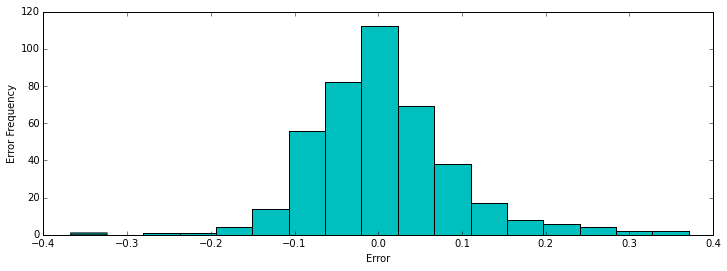
\includegraphics[width=\textwidth]{baseline1_error_histogram.png}
\caption{Error plot for baseline model - oil/gold price is the same as the previous month's price}
\label{fig:baseline1_error_histogram.png}
\end{figure}

\begin{table}
\begin{center}
\begin{tabular}{|c|c|c|c|}
\hline
Model & Relative Error & Mean Absolute Error & Root Mean Squared Error \\ \hline
$ Model 0.0 $ & $3.674560$ & $29.142500$ & $49.049942$ \\ \hline
$ Model 0.1 $ & $3.606751$ & $28.856644$ & $47.804751$\\ \hline
\end{tabular}
\end{center}
\caption{Error Metrics for Baseline Model - Gold}
\end{table}


\begin{figure}
\centering
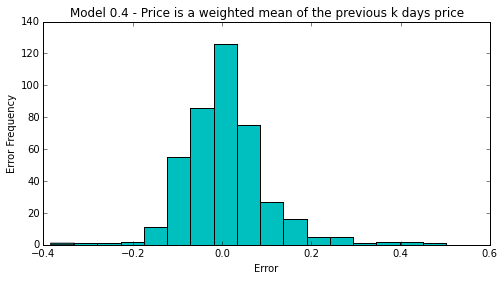
\includegraphics[width=\textwidth]{baseline2_error_histogram.png}
\caption{Error plot for baseline model - oil/gold price is a weighted mean of price of previous k months}
\label{fig:baseline2_error_histogram.png}
\end{figure}

\subsection{Spot price prediction using futures prices}

A futures contract is an agreement between two parties to buy or sell a specific asset at a time in the future for a price decided today \cite{futures_book}. One party takes a long position - it agrees to buy the asset or commodity, and the other party takes a short position - it agrees to sell the same asset or commodity. The purpose of these contracts is to hedge risks.\\

\noindent A futures market is a financial exchange where futures contracts are traded. If there are more sellers than buyers, which is indicative of a reduction in demand of a particular asset, the futures prices of that asset go down. However, more number of buyers than sellers indicates that the supply is unable to meed the demands, which results in an increase in the price of that asset. \\

\noindent Most futures contracts do not lead to delivery because traders choose to close out their positions prior to delivery, however it is this factor that ties the futures price to the spot prices. \\

\noindent Commodities such as oil and gold are also traded on the futures market. The are are two types of assets - investment assets and consumption assets. Gold is considered as an investment asset and has a net income associated with it. Oil is a consumption asset and has storage costs associated.\\

\noindent The value of the futures contracts and the futures prices of oil and gold hold some information in them which can help us determine the price of these commodities.  

\newpage
\section{Data Matrices}
Our data consists of multiple time series of monthly Oil and Gold prices\cite{quandal}, and the following macroeconomic factors:

\begin {itemize}
\item S\&P 500 Index \cite{quandal}
\item New York Stock Exchange Index (NYSE) \cite{quandal}
\item US Dollar Index \cite{quandal}
\item Consumer Sentiment Index (CSI) \cite{csi}
\item EURO-USD Conversion Rate \cite{quandal}
\end {itemize}
 
\begin{figure}
\centering
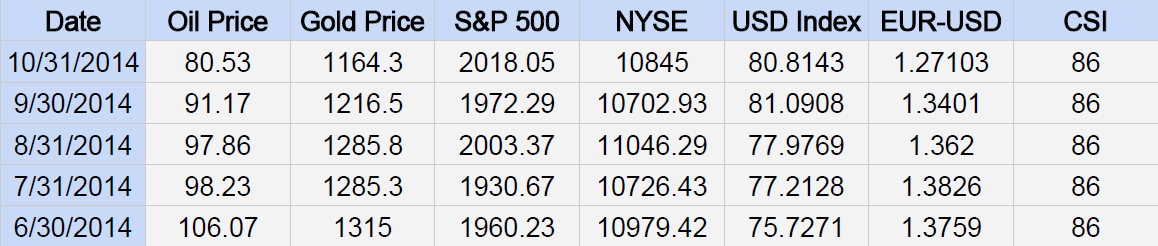
\includegraphics[width=\textwidth]{DataMatrices.png}
\caption{Data frame for oil and gold price and its related macroeconomic factors}
\label{fig:DataMatrices.png}
\end{figure}

\begin{figure}
\centering
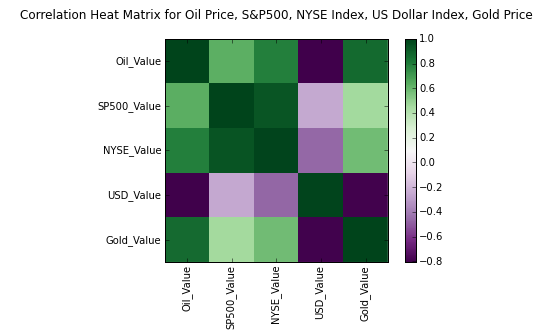
\includegraphics[width=\textwidth]{HeatMap_Oil_Monthly.png}
\caption{Correlation Heat Map for Oil Price and related macroeconomic factors}
\label{fig:HeatMap_Oil_Monthly.png}
\end{figure}

\begin{table}
\begin{center}
\begin{tabular}{|c|c|c|c|c|}
\hline
$ $ & $ S\&P\ 500 $ & $ NYSE $ & $ USD\ Index $ & $Gold\ Price$ \\ \hline
$Oil Price$ & $0.718178$ & $0.805763$ & $-0.77365$ & $0.872$ \\ \hline
\end{tabular}
\end{center}
\caption{Correlation Matrix - Oil}
\end{table}


The correlation heat map in \autoref{fig:HeatMap_Oil_Monthly.png}, and the corresponding table containing correlation coefficients show the correlation between the price of oil and related economic factors. They indicate a high correlation between oil price and certain macroeconomic factors - S\&P 500, NYSE, US Dollar Index, Gold Price.

\begin{figure}
\centering
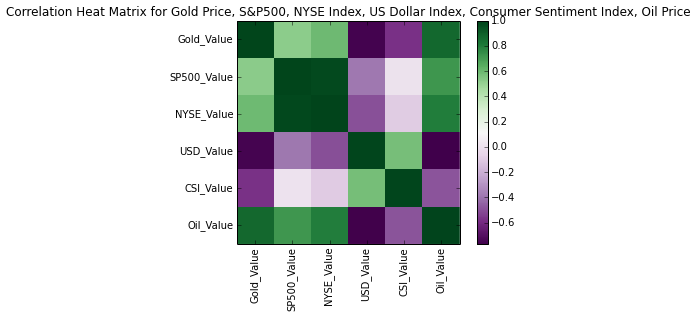
\includegraphics[width=\textwidth]{HeatMap_Gold_Monthly.png}
\caption{Correlation Heat Map for Oil Price and related macroeconomic factors}
\label{fig:HeatMap_Gold_Daily.png}
\end{figure}

\begin{table}
\begin{center}
\begin{tabular}{|c|c|c|c|c|c|c|}
\hline
$ $ & $ S\&P 500 $ & $ NYSE $ & $ USD $ & $EUR-USD$ & $CSI$ &$Oil Price$ \\  \hline
$Gold Price$ & $0.461485$ & $0.578967$ & $-0.792106$ & $0.628074$ & $-0.727766$ & $0.860482$ \\ \hline
\end{tabular}
\end{center}
\caption{Correlation Matrix - Gold}
\end{table}

The correlation heat map in \autoref{fig:HeatMap_Gold_Daily.png}, and the corresponding table containing correlation coefficients show the correlation between the price of oil and related economic factors. They indicate a high correlation between Gold Price and certain macroeconomic factors - US Dollar Index, EURO-USD Conversion Rate and Oil Price.\\

\noindent Our goal is to predict the prices of oil and gold on January 1st, 2015 as of December 1st, 2014, which is a month in advance. Therefore, we have used monthly data, i.e, oil/gold price and values of other economic factors on the last day of every month. But this severely limits the amount of data we can obtain. Although we collected data for the past 30 years, we have just 360 entries in our time series, which isn't a good enough number to generate good enough error metrics. This also limits our prediction power. \\

\newpage
\section{Development/Evaluation Environment}

\begin{figure}
\centering
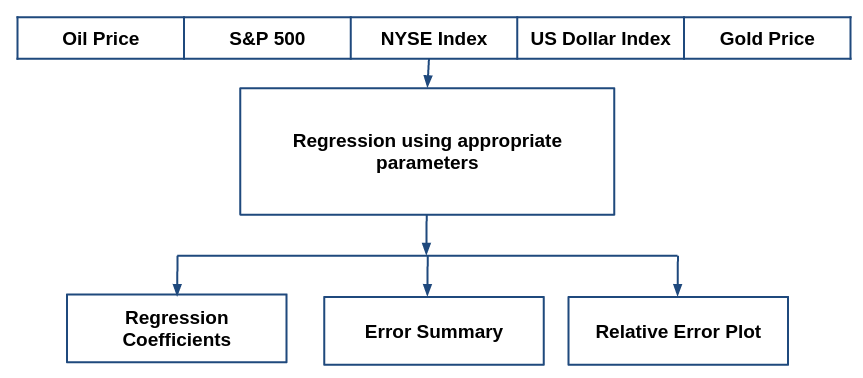
\includegraphics[width=\textwidth]{DevelopmentFlowchart.png}
\caption{The development and evaluation environment for the oil/gold price prediction with economic factors involved}
\label{fig:DevelopmentFlowchart.png}
\end{figure}

\noindent \autoref{fig:DevelopmentFlowchart.png} shows the workflow of our prediction model. The model uses past prices of oil/gold, combined with certain macroeconomic factors, and performs regression to make predictions. Error metrics are used to determine the accuracy of our predictions.\\

\noindent The model takes a data frame containing multiple time series of oil/gold prices and related macroeconomic factors as an input. A parameter corresponding to each of these factors is also passed as a part of the input to the model. This parameter is an integer representing the number of lags in the autoregressive factor, and is used to predict the current value of the time series. We can also choose not to consider a particular factor by assigning $0$ to the parameter.\\

\noindent The model is trained on the initial 60\% of the time series, and tested on the remaining 40\%. It tries to generate a linear function while assigning coefficients to each of these economic factors. These regression coefficients are then used to make predictions for the next month. In order to ensure that that our model does not over-fitting the curve, our time series is cross validated using a size $k$ slice of from training set($k$ is nearly equal to 80\%). This slice is then slid across the training set, and finally an average of the different predictions of each slice is calculated. However, since there was no improvement in the results, we did not incorporate it as a part of our model.\\

The Mean Relative Error, Mean Absolute Error, and Root Mean Square Error are calculated, and a histogram of the relative error frequencies is generated. \\

\newpage
\section{Current Model and Baseline}

We have developed autoregressive and multiple linear regressive models to make oil and gold price predictions.

\subsubsection{Autoregressive Model}
Autoregressive models are based purely on historical prices. They model the time series as a linear function of the values of the past 'p' months.\\

$ X_{t} = c + \sum\limits_{i=1}^p \varphi_{t-i}X_{t-i}$. \\

\noindent The Ordinary Least Squares (OLS) method is used to estimate the parameters of the regression function. It tries to minimize the sum of squares of vertical distances between the predicted and the actual values. 

\subsubsection{Autoregressive and Multiple Linear Regressive Model}
Linear regression models the relationship between two variables - a dependent variable and an explanatory variable using a linear function. The process of modelling a variable based on more than one explanatory variables is called Multiple Linear Regression. \\
   
\noindent We initially develop a model which generates a purely autoregressive function. Then, the model is expanded to incorporate the factors which are highly correlated to the price of oil/gold we are trying to predict. As each factor is incorporated into the model, we perform a comparison of the error metrics between these models and try to estimate the model which makes predictions with a better accuracy.\\

For predicting the price of oil, the following macroeconomic factors are taken into consideration:
\begin {itemize}
\item S\&P 500 Index
\item NYSE Index
\item US Dollar Index
\item Gold Price
\end {itemize}

For predicting the price of gold, the following factors macroeconomic are taken into consideration:
\begin {itemize}
\item S\&P 500 Index
\item NYSE Index
\item US Dollar Index
\item EURO-USD Exchange Rate
\item Consumer Sentiment Index
\item Oil Price
\end {itemize}


\subsubsection{Autoregressive Moving Average Model (ARMA)}
ARMA models are used to understand and predict time series values as a function of two polynomials, an autoregressive function, and a moving average function. 
\\

$ X_{t} = c + \sum\limits_{i=1}^p \varphi_{t-i}X_{t-i} + \epsilon_{t} + \sum\limits_{i=1}^q \theta_{t-i}X_{t-i}$.\\

In ARMA (p,q), p is referred to as the order of the autoregressive part and q is referred to as the order of the moving average part, i.e, the model is described using p autoregressive terms and q moving average terms.\\ 

\subsubsection {Why other autoregressive models fail to perform much better than baseline?}
ACF: Autocorrelation Factor
PACF: Partial autocorrelation Factor(auto-correlation with the linear dependence between variables removed)
\\

[ADD]
\subsection {OIL}

\subsubsection {Autoregressive and Multiple Linear Regression Models}.\\

We initially try to predict the price of oil solely on the basis of the past values of oil prices. \autoref{fig:oil_autoregressive.png} shows the performance of the autoregressive model as the number of months taken into consideration by the model is increased. \\

\begin{figure}
\centering
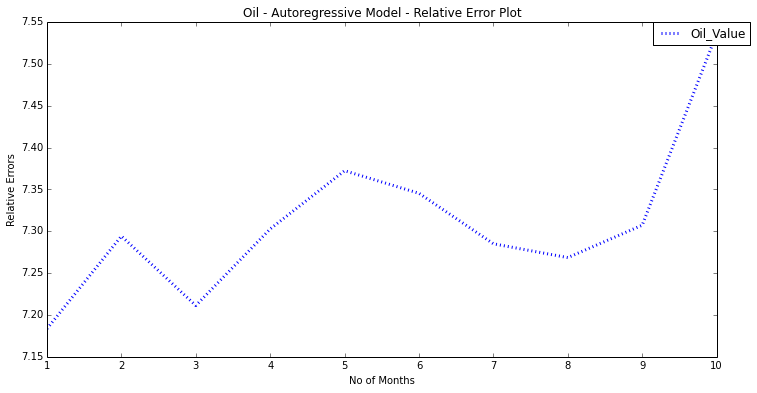
\includegraphics[width=\textwidth]{oil_autoregressive.png}
\caption{Performance of the autoregressive model with increasing number of months}
\label{fig:oil_autoregressive.png}
\end{figure}

We then incorporate the macroeconomic factors into the model. We start by including one factor at a time to the autoregressive model and use the error metrics to compare the performance of these models. For each of these models, we plot a graph of the relative error against the number of months taken into consideration. \autoref{fig:oil_autoregressive_1factor_10.png}, \autoref{fig:oil_autoregressive_2factors_10.png}, and \autoref{fig:oil_autoregressive_3factors_10.png} show the error plots for different models. 

\begin{figure}
\centering
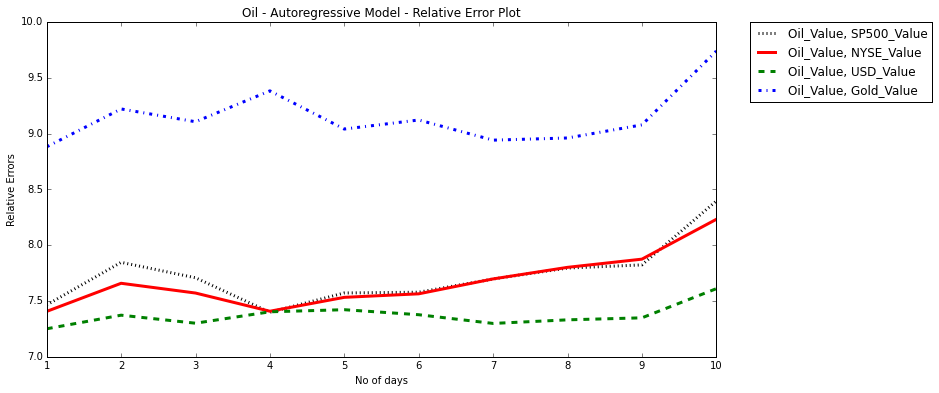
\includegraphics[width=\textwidth]{oil_autoregressive_1factor_10.png}
\caption{Performance of the autoregressive model considering one factor with increasing number of months}
\label{fig:oil_autoregressive_1factor_10.png}
\end{figure}

\begin{figure}
\centering
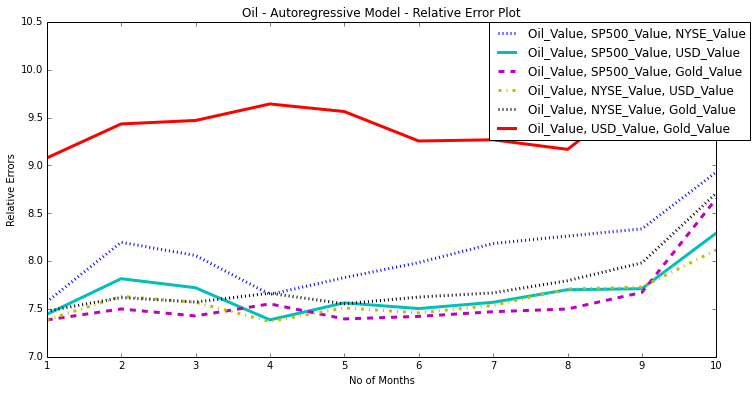
\includegraphics[width=\textwidth]{oil_autoregressive_2factors_10.png}
\caption{Performance of the autoregressive model considering two factors with increasing number of months}
\label{fig:oil_autoregressive_2factors_10.png}
\end{figure}

\begin{figure}
\centering
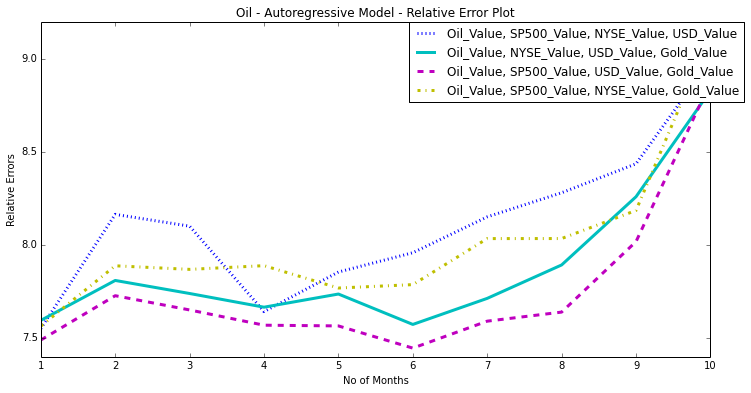
\includegraphics[width=\textwidth]{oil_autoregressive_3factors_10.png}
\caption{Performance of the autoregressive model considering 3 factors with increasing number of months}
\label{fig:oil_autoregressive_3factors_10.png}
\end{figure}

\newpage
\subsubsection {ARMA Model}.\\

\noindent We also developed an ARMA(p,q) model to predict the price of oil. After testing the ARMA model with various values of p and q, we observed that the ARMA (6,0) model was giving us the best results for predicting the oil price.  \\

\noindent \autoref{fig:arma_autocorrelation.png} shows a plot of the autocorrelation and the partial autocorrelation factors between the prices of oil over the past 40 days. \\

\noindent \autoref{fig:arma_error_histogram.png} shows a typical relative error distribution of the ARMA model.

\begin{center}
\begin{figure}
\centering
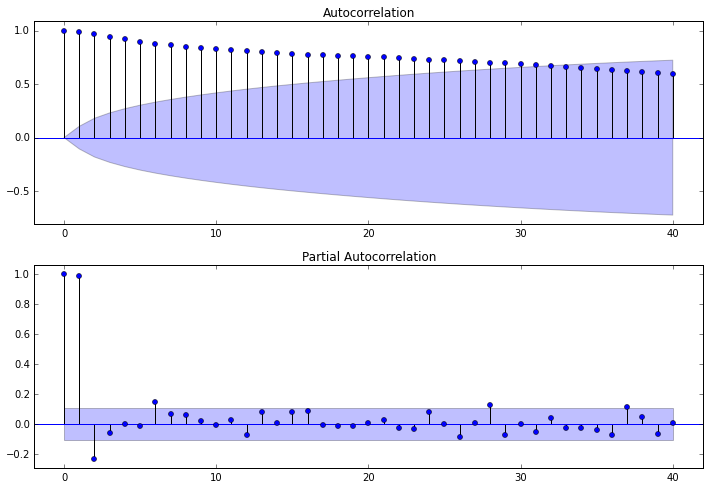
\includegraphics[width=\textwidth]{arma_autocorrelation.png}
\caption{ARMA Autocorrelation and Partial Autocorrelation factors}
\label{fig:arma_autocorrelation.png}
\end{figure}
\end{center}

\begin{figure}
\centering
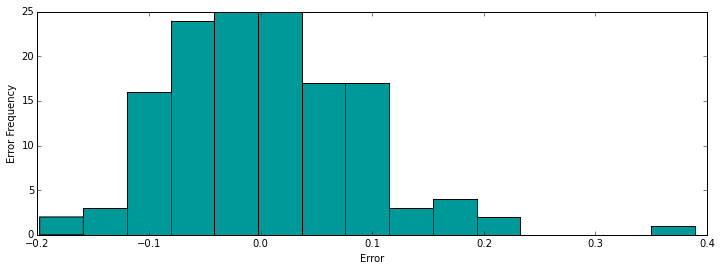
\includegraphics[width=\textwidth]{arma_error_histogram.png}
\caption{ARMA Error Distribution}
\label{fig:arma_error_histogram.png}
\end{figure}

\newpage
\subsubsection {Comparison Summary - Oil} The following is a summary of the comparison between autoregressive and multiple linear regressive models against the baseline models. \\

\begin{figure}
\centering
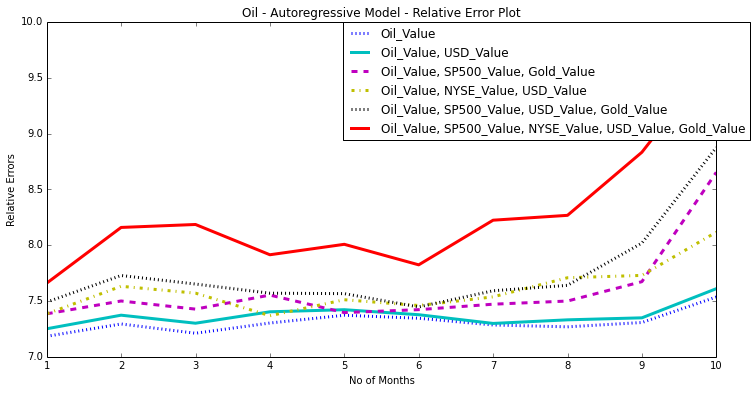
\includegraphics[width=\textwidth]{oil_autoregressive_bestModels.png}
\caption{Best performing models for predicting oil prices}
\label{fig:oil_autoregressive_bestModels.png}
\end{figure}

\autoref{fig:oil_autoregressive_bestModels.png} shows a comparison of the best performing models considering various econometric factors.


\begin{figure}
\centering
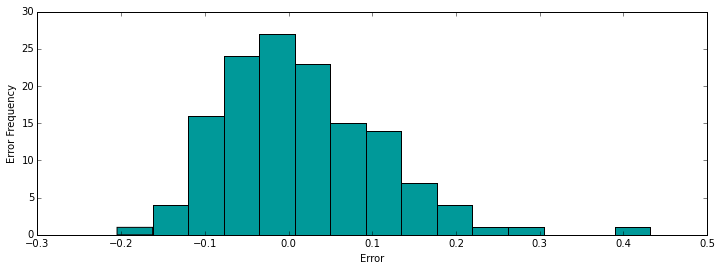
\includegraphics[width=\textwidth]{oil_autoregressive_error_histogram.png}
\caption{Typical error distribution of an autoregressive and multiple linear regressive model}
\label{fig:oil_autoregressive_error_histogram.png}
\end{figure}

\autoref{fig:oil_autoregressive_error_histogram.png} shows a typical error distribution of an autoregressive and multiple linear regressive model.


\begin{table}
\begin{center}
\begin{tabular}{|c|c|c|c|}
\hline
Factors & Relative Error & Mean Abs Error & RMSE\\ \hline \hline 
$ Baseline Model 0.0 $ & $6.73746$ & $5.384215$ & $7.101763$ \\ \hline
$ Baseline Model 0.1 $ & $7.27174$ & $5.761054$ & $7.754635$\\ \hline
$ Autoregressive $ & $8.49$ & $5.097663$ & $6.672619$ \\ \hline
$ USD\ Index $ & $8.69$ & $5.137571$ & $6.67896$\\ \hline
$ S\&P500,\ Gold\ Price $ & $9.04$ & $5.160815$ & $6.737639$\\ \hline
$ NYSE,\ USD$ & $9.05$ & $5.241797$ & $6.767898$\\ \hline
$ S\&P500,\ USD,\ Gold\ Price $ & $9.38$ & $5.26046$ & $6.79724$\\ \hline
$ S\&P500,\ NYSE,\ USD,\ Gold\ Price $ & $10.86$ & $5.494503$ & $7.000936$\\  \hline
$ ARMA\ (6,0) $ & $5.0322462866$ & $6.42218763098$ & $6.78951497738$\\  \hline

\end{tabular}
\end{center}
\caption{Summary of error metrics of various models for predicting oil prices}
\end{table}

\newpage
\subsection {GOLD}

\subsubsection {Autoregressive and Multiple Linear Regression Models}.\\

We follow a similar procedure for gold - we initially try to predict the price of gold solely on the basis of historical gold prices. We then add one economic factor at a time, compare the different models obtained to derive the best performing model. We only include factors with absolute correlation coefficients equal or greater than 0.55 with the gold price. Hence, we discard S\&P500 for gold.


\noindent \autoref{fig:gold_autoregressive.png} shows the performance of the autoregressive model as the number of months taken into consideration by the model is increased. \\

\begin{figure}
\centering
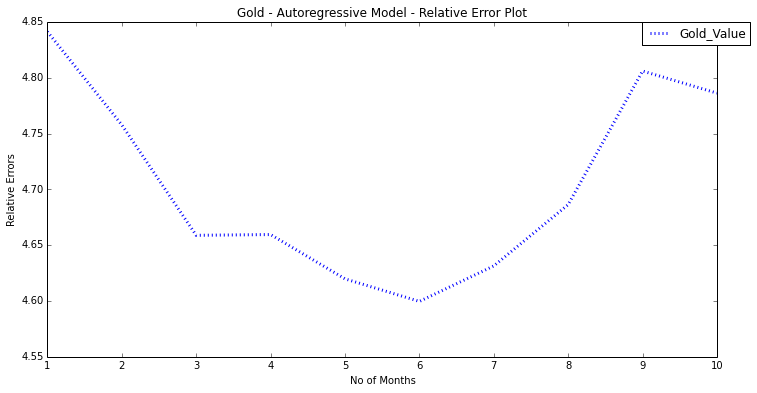
\includegraphics[width=\textwidth]{gold_autoregressive.png}
\caption{Performance of the autoregressive model with increasing number of months}
\label{fig:gold_autoregressive.png}
\end{figure}

\begin{figure}
\centering
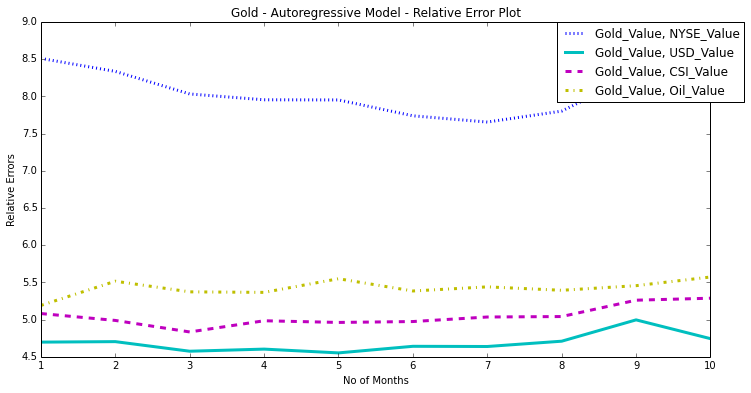
\includegraphics[width=\textwidth]{gold_autoregressive_1factor_10.png}
\caption{Performance of the autoregressive model considering one factor with increasing number of months}
\label{fig:gold_autoregressive_1factor_10.png}
\end{figure}

\begin{figure}
\centering
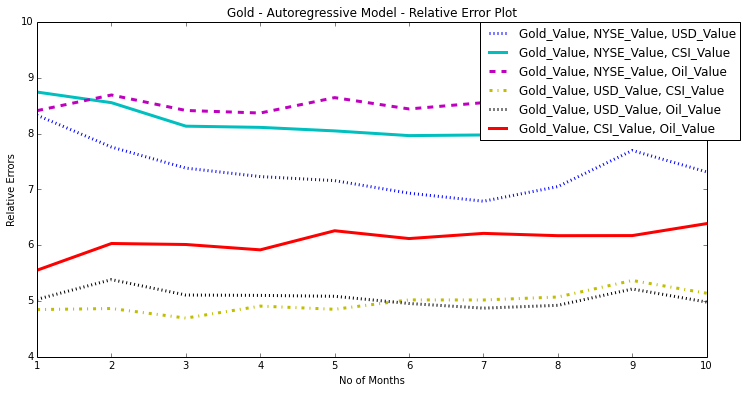
\includegraphics[width=\textwidth]{gold_autoregressive_2factors_10.png}
\caption{Performance of the autoregressive model considering two factors with increasing number of months}
\label{fig:gold_autoregressive_2factors_10.png}
\end{figure}

\begin{figure}
\centering
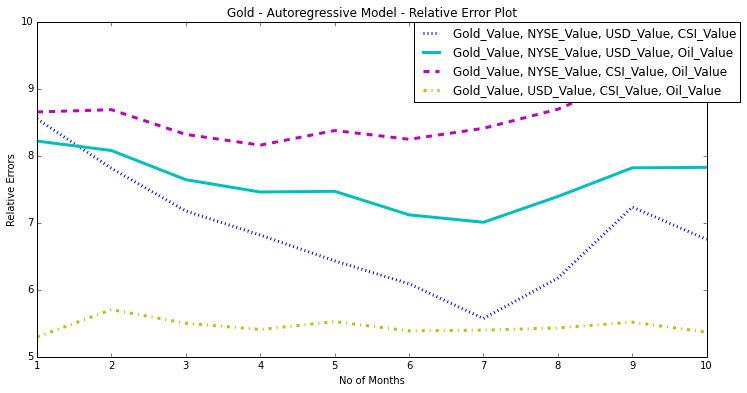
\includegraphics[width=\textwidth]{gold_autoregressive_3factors_10.png}
\caption{Performance of the autoregressive model considering three factors with increasing number of months}
\label{fig:gold_autoregressive_3factors_10.png}
\end{figure}

\noindent \autoref{fig:gold_autoregressive_1factor_10.png}, \autoref{fig:gold_autoregressive_2factors_10.png}, and \autoref{fig:gold_autoregressive_3factors_10.png} show the error plots for different models. 

\newpage
\newpage
\subsubsection {ARMA Model}.\\

Similar to oil, the ARMA model was also used to predict gold prices. Here, we observed that ARMA (2,0) was giving us the best results.

\begin{center}
\begin{figure}
\centering
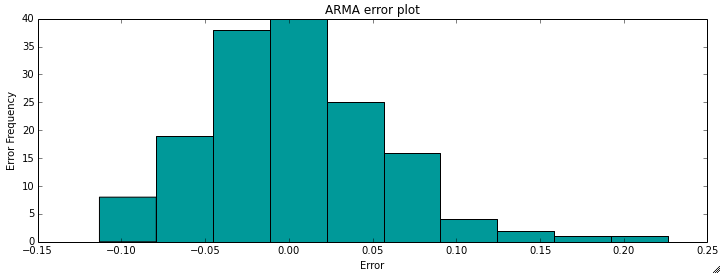
\includegraphics[width=\textwidth]{arma_error_histogram_gold.png}
\caption{ARMA Error Distribution}
\label{fig:arma_error_histogram_gold.png}
\end{figure}
\end{center}


\noindent \autoref{fig:arma_error_histogram_gold.png} shows a typical relative error distribution of the ARMA model.

\begin{center}
\begin{figure}
\centering
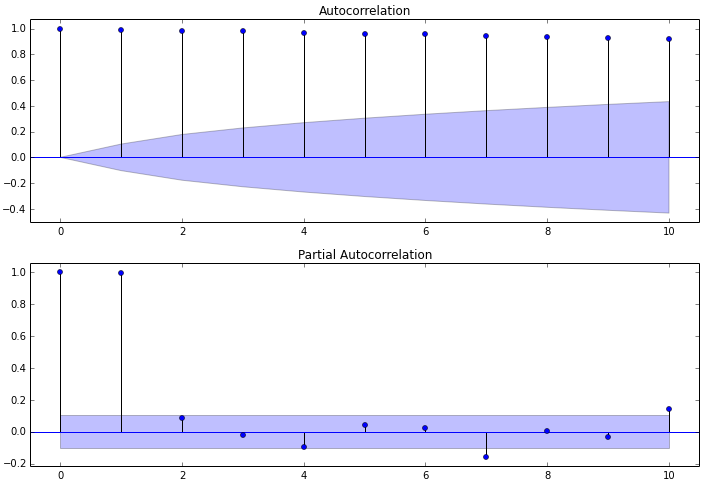
\includegraphics[width=\textwidth]{arma_autocorrelation_gold.png}
\caption{ARMA Autocorrelation and Partial Autocorrelation factors}
\label{fig:arma_autocorrelation_gold.png}
\end{figure}
\end{center}

\noindent \autoref{fig:arma_autocorrelation_gold.png} shows a plot of the autocorrelation and the partial autocorrelation factors between the prices of oil over the past 10 days. \\


\newpage
\subsubsection {Comparison Summary - Gold} The following is a summary of the comparison between autoregressive and multiple linear regressive models against the baseline models. \\


\begin{figure}
\centering
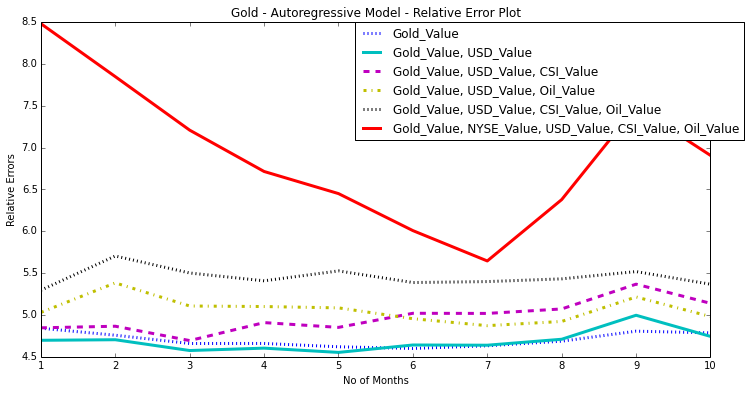
\includegraphics[width=\textwidth]{gold_autoregressive_bestModels.png}
\caption{Best performing models for predicting oil prices}
\label{fig:gold_autoregressive_bestModels.png}
\end{figure}

\autoref{fig:gold_autoregressive_bestModels.png} shows a comparison of the best performing models.

\begin{figure}
\centering
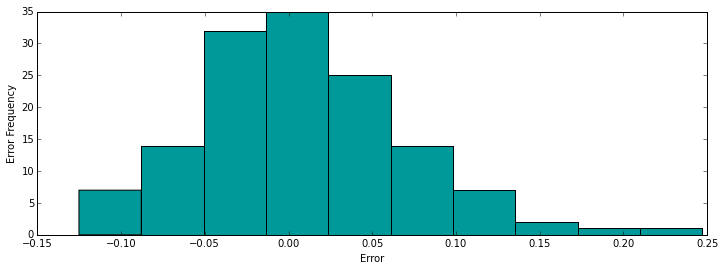
\includegraphics[width=\textwidth]{gold_autoregressive_error_histogram.png}
\caption{Typical error distribution of an autoregressive and multiple linear regressive model}
\label{fig:gold_autoregressive_error_histogram.png}
\end{figure}

\autoref{fig:gold_autoregressive_error_histogram.png} shows a typical error distribution of an autoregressive and multiple linear regressive model.

\begin{table}
\begin{center}
\begin{tabular}{|c|c|c|c|}
\hline
Factors & Relative Error & Mean Abs Error & RMSE\\ \hline \hline 
$ Baseline\ Model\ 0.0 $ & $3.674560$ & $29.142500$ & $49.049942$ \\ \hline
$ Baseline\ Model\ 0.1 $ & $3.606751$ & $28.856644$ & $47.804751$\\ \hline
$ Autoregressive $ & $4.82$ & $44.65614$ & $62.92901$ \\ \hline
$ USD\ Index $ & $4.82$ & $44.14099$ & $62.53696$\\ \hline
$ USD\ Index,\ CSI $ & $5.07$ & $45.46891$ & $63.04931$\\ \hline
$ USD\ Index,\ Oil\ Price$ & $5.25$ & $46.82992$ & $63.24664$\\ \hline
$ USD\ Index,\ CSI,\ Oil\ Price $ & $5.71$ & $49.1547$ & $64.68856$\\ \hline
$ NYSE,\ USD\ Index,\ CSI,\ Oil\ Price $ & $6.72$ & $53.99127$ & $67.96092$\\  \hline
$ ARMA\ (2,0) $ & $4.24125955354$ & $40.5505169891$ & $58.9195927119$\\  \hline

\end{tabular}
\end{center}
\caption{Summary of error metrics of various models predicting gold prices}
\end{table}


\newpage
\section{Current Prediction and Next Steps}

\subsection {Current Prediction}
\noindent The predicted price of WTI Crude Oil on Dec 1 as of Nov 1 is \\
\textbf{00.00 USD per Barrel} \\

\noindent The predicted price of Gold on Dec 1 as of Nov 1 \\
\textbf{0000.00 USD per ounce} \\

\subsection {Next Steps}

\begin{itemize}
\item \textbf{Better Models} We need to improve our model  
\item \textbf{Futures} We need to figure out how the futures prices can give us more information about the price of a commodity.
 
\end{itemize}

[ADD "Present what you will do next to get a complete predictive model.  Discuss any difficulties you will have to overcome in building a good model"]

\subsubsection*{Acknowledgments.} Here acknowledge any other people who helped with this project.

\section{Bibliography}\label{references}

\begin{thebibliography}{4}

\bibitem{futures_book} Hull, John. Options, futures and other derivatives. Pearson education, 2009.

\bibitem{quandal} Quandl - Find, Use and Share Numerical Data. \url{https://www.quandl.com}

\bibitem{csi}\url{http://future.aae.wisc.edu/data/monthly_values/by_area/998?grid=true}

\end{thebibliography}


\end{document}
